\documentclass[10pt,xcolor={usenames}]{beamer}
\usepackage{beamerthemesplit}
\usetheme{madrid}
%\usecolortheme{crane}

\usepackage[T2A]{fontenc}
%\usepackage[cp1251]{inputenc} %for Windows
\usepackage[utf8]{inputenc}

%\documentclass[a4paper, 1wpt]{amsart}
\usepackage[english]{babel}

\usepackage{cmap}
\usepackage{amsfonts, amssymb, amscd, amsmath}
\usepackage{latexsym}
\usepackage[matrix,arrow,curve]{xy}
\usepackage{mathabx}%,mathtools}
%\usepackage{color}

\usepackage{graphics}
\usepackage{graphicx}
 \usepackage{color}
 \usepackage{transparent}
%\usepackage[dvipsnames]{xcolor}

\usepackage{pbox}
\usepackage{tikz}
\usepackage{array}
%\usetikzlibrary{matrix,decorations.pathreplacing,positioning}
%\usepackage{scalerel}
\usepackage{hyperref}

\usepackage{parskip}
\usepackage{array}
\usepackage{epigraph}
\usepackage{animate}
\usepackage{stackrel}

%\DeclareSymbolFont{cyrillic}{T2A}{cmr}{m}{n}
%\DeclareMathSymbol{\Tse}{\mathalpha}{cyrillic}{214}


\newcolumntype{M}[1]{>{\centering\arraybackslash}m{#1}}

%\renewcommand{\contentsname}{GGGGGGGGGGGGG}

\definecolor{emph}{RGB}{200,90,0}

\newcolumntype{P}[1]{>{\centering\arraybackslash}p{#1}}

\newcommand*\circled[1]{\tikz[baseline=(char.base)]{
            \node[shape=circle,draw,inner sep=2pt] (char) {#1};}}

\DeclareMathOperator{\Cone}{Cone}
\DeclareMathOperator{\pt}{pt}
\DeclareMathOperator{\Ker}{Ker}
\DeclareMathOperator{\id}{id}
\DeclareMathOperator{\codim}{codim}
\DeclareMathOperator{\sgn}{sgn}
\DeclareMathOperator{\Imm}{Im}
\DeclareMathOperator{\im}{Im}
\DeclareMathOperator{\supp}{supp}
\DeclareMathOperator{\const}{const}
\DeclareMathOperator{\Hom}{Hom}
\DeclareMathOperator{\rk}{rk}
\DeclareMathOperator{\diag}{diag}
\DeclareMathOperator{\conv}{conv}
\DeclareMathOperator{\tr}{tr}
\DeclareMathOperator{\re}{Re}
\DeclareMathOperator{\PH}{PH}
\DeclareMathOperator{\EMST}{EMST}
\DeclareMathOperator{\LMST}{LMST}
\DeclareMathOperator{\Hilb}{P}
\DeclareMathOperator{\PD}{PD}

\DeclareMathOperator{\Sym}{Sym}

\DeclareMathOperator{\low}{low}

\DeclareMathOperator{\nc}{nc}


\DeclareMathOperator{\dist}{dist}
\DeclareMathOperator{\grad}{grad}

\newcommand{\ko}{\Bbbk}
\newcommand{\Fo}{\mathbb{F}}
\newcommand{\Zo}{\mathbb{Z}}
\newcommand{\Ro}{\mathbb{R}}
\newcommand{\Rg}{\mathbb{R}_{\geqslant 0}}
\newcommand{\Co}{\mathbb{C}}
\newcommand{\Qo}{\mathbb{Q}}
\newcommand{\Noo}{\mathbb{N}}
\newcommand{\Zt}{\Zo_2}
\newcommand{\Eo}{\mathbb{E}}

\newcommand{\br}{\widetilde{\beta}}
\newcommand{\eqd}{\stackrel{\text{\tiny def}}{=}}
\newcommand{\toiso}{\stackrel{\cong}{\to}}

\newcommand{\wh}[1]{{\widehat{#1}}}
\newcommand{\ca}[1]{\mathcal{#1}}

\newcommand{\Ch}{\check{C}}

\newcommand{\Hr}{\widetilde{H}}
\newcommand{\dd}{\partial}
\newcommand{\Ca}{\mathcal{C}}
\newcommand{\F}{\mathcal{F}}


\newcommand{\RP}{\mathbb{R}P}
\newcommand{\CP}{\mathbb{C}P}


\title[Topology intro]{Topological data analysis \\ Lecture 4}
\author[Anton Ayzenberg]{ Anton Ayzenberg }% \\  \texttt{ayzenberga@gmail.com}}
\date[FCS-YDS'24]{Spring 2024 \\ Faculty of Computer Science / Yandex Data School}
\institute[ATA \& Noeon Research]{ATA Lab, FCS NRU HSE \\ Noeon Research}

\begin{document}

\maketitle


\begin{frame}{A principal incompatibility between ``topology'' and ``applied''.}

\begin{itemize}
  \item Data analysis and machine learning deal with real numbers and real optimization.
  \item Topological invariants are discrete. There is no space with $2.3457$ many connected components or $\frac{5}{6}$ many holes.
  \item How can one make Topology ``applied''?
\end{itemize}
\pause

\begin{block}{Introduce ``topological processes''!}
Let $X_t$ be a space depending on time $t\in\Ro$. If $t_1\leq t_2$, we assume there is a map
\[
f_{t_1\leqslant t_2}\colon X_{t_1}\to X_{t_2},
\]
such that $f_{t\leqslant t}=\id_{X_t}$ and $f_{t_2\leqslant t_3}\circ f_{t_1\leqslant t_2}=f_{t_1\leqslant t_3}$.
\end{block}

Compare this with stochastic processes...

\end{frame}


\begin{frame}{Idea of applied topology}

\begin{block}{Topological process}
Let $X_t$ be a space depending on time $t\in\Ro$ and there are maps $f_{t_1\leqslant t_2}\colon X_{t_1}\to X_{t_2}$.
\end{block}

Usually, all connecting maps $f_{t_1\leqslant t_2}$ are inclusions. In this case the process is called a \textbf{filtration}.

\begin{block}{Idea}
\begin{itemize}
  \item We may average topological invariants along all values of time $t$.
  \item This gives real-valued invariants which can be optimized using methods of machine learning.
\end{itemize}
\end{block}

\end{frame}

\begin{frame}{Important construction}

\begin{block}{Sublevel set filtration}
Let $f\colon \Ro^d\to \Ro$ be a function. Consider sublevel sets of $f$
\[
X^f_t=\{x\in \Ro^d\mid f(x)\leqslant t\}
\]
This is a filtration.
\end{block}

\begin{center}
  \includegraphics[scale = 0.13]{pictures/sublevel.pdf}
\end{center}

\end{frame}

\begin{frame}{Another important construction}

\begin{block}{\v{C}ech filtration}
Let $X=\{x_1,\ldots,x_m\}\subset \Ro^d$ be a finite set (point cloud). Itself, the space $X$ is not interesting topologically. But we may surround each point with a ball of variable radius $t/2$, and see how topology evolve:
\[
X_t=\bigcup_{i=1}^m B_{t/2}(x_i)
\]
This is a filtration defined for $t\geqslant 0$.
\end{block}

\end{frame}

\begin{frame}{\v{C}ech filtration}

\begin{center}
  \includegraphics[scale = 0.14]{pictures/sampling.pdf}
\end{center}

\end{frame}

\begin{frame}{Toy example: average number of components}

Let $X=\{x_1,\ldots,x_m\}\subset \Ro^d$ be a point cloud and $X_t$ its \v{C}ech filtration. Let $\nc(X_t)$ be the number of connected components of $X_t$.

\begin{block}{A new invariant}
Define the number
\[
\overline{\nc}(X)=\int_{0}^{+\infty} (\nc(X_t)-1)dt.
\]
\end{block}
\pause

Question: any guess what $\overline{\nc}(X)$ is?

\begin{center}
Demonstration: \href{https://play.unity.com/mg/other/builds-4z-1}{press to play in browser}
\end{center}

\end{frame}

\begin{frame}{Toy example: evolution of components}

\begin{block}{Answer:}
$\overline{\nc}(X)$ equals the length of the minimal spanning tree of $X$. Guess why.
\end{block}

\pause

\begin{center}
  Dendrogram \includegraphics[scale = 0.3]{pictures/dendrogram.pdf}
\end{center}

Open question: how can we encode such dendrograms?

\end{frame}

\begin{frame}{Persistent homology}

\begin{block}{Homology}
Homology = higher dimensional analogue of counting connected components. $\beta_i(X)$ = number of $i$-dimensional holes in $X$.  
\end{block}

\begin{block}{Persistent homology}
How the number of holes in a filtration changes in time.
\end{block}

\end{frame}
%
%\begin{frame}{Today's lesson}
%
%My plan for the rest of this lecture and for the seminar: estimation of dimension.
%
%\textcolor{red}{Problem:} given a finite point-set $X\subset \Ro^d$, estimate its intrinsic dimension.
%
%\begin{enumerate}
%  \item Linear method: PCA.
%  \item \textbf{Nonlinear dimension estimation. }
%\end{enumerate}
%
%Approach: use length of minimal spanning tree (LMST).
%
%\end{frame}
%
%\begin{frame}{LMST for point clouds in $\Ro^d$}
%
%Assume that $x_i$, $i=1,\ldots,n$ are sampled independently from a continuous distribution on $k$-dimensional manifold $M^k\subset \Ro^d$.
%\begin{itemize}
%  \item $d$ : ambient dimension.
%  \item $k$ : intrinsic dimension.
%\end{itemize}
%
%\begin{block}{Theorem (Steele'88)}
%\[
%\LMST(A_n)\sim C_k n^{\frac{k-1}{k}}\mbox{ when } n\to\infty.
%\]
%\end{block}
%
%This gives a \textcolor{blue}{fractal-type} formula to estimate the \textcolor{red}{intrinsic dimension} from the point cloud:
%\[
%\dfrac{k-1}{k} = \beta = \lim_{n\to\infty}\dfrac{\log \LMST(A_n)}{\log n},
%\]
%hence $k=\dfrac{1}{1-\beta}$.
%\end{frame}
%
%
%\begin{frame}{Example}
%
%What is the intrinsic dimension in this case? PCA tells it is 2.
%
%\begin{center}
%  \includegraphics[scale = 0.5]{pictures/cloud1.pdf}
%\end{center}
%
%\end{frame}
%
%\begin{frame}{Example}
%
%What is the intrinsic dimension in this case? LMST tells it is closer to 0.
%
%\begin{center}
%  \includegraphics[scale = 0.5]{pictures/cloud2.pdf}
%\end{center}
%
%\end{frame}
%
%
%
%\begin{frame}{Erd\H{o}s--R\'{e}nyi metric graph}
%
%What if data are not chosen in $\Ro^n$ but rather take the form of a random metric graph?
%
%\begin{block}{Construction}
%Let us take $n$ points and set pairwise distances $d_{i,j}$ independently uniformly from $[0;1]$. Denote this \textcolor{red}{random metric graph} by $\Gamma_n$.
%\end{block}
%
%\begin{block}{General problem}
%What can we say about LMST of $\Gamma_n$?
%\end{block}
%
%%\href{https://colab.research.google.com/drive/146yQdZBsPGfYZwi1AGKJwSE5wjRwPnc1?usp=sharing}{Experiments}: sum of lifetimes of $\PH_0(K_t^{VR}(\Gamma_n))$ is around $1.2$ and does not grow with $n$.
%
%\end{frame}
%
%
%\begin{frame}{Experiments}
%
%\begin{center}
%  \includegraphics[scale = 0.5]{pictures/LMSTexperiment.png}
%\end{center}
%
%\[
%\mbox{\textcolor{purple}{Why this number is not growing?}}
%\]
%\pause
%\[
%\mbox{\textcolor{purple}{Do you recognize the number 1.2?}}
%\]
%\end{frame}
%
%
%\begin{frame}{Ap\^{e}ry's constant}
%
%\[
%\zeta(3)=\sum_{n=1}^{\infty}\dfrac{1}{n^3}\approx 1.20205
%\]
%
%\begin{block}{Theorem (Frieze'85)}
%Let $\LMST_n$ be the length of the MST for the random graph $\Gamma_n$.
%\begin{enumerate}
%  \item $\lim\limits_{n\to\infty} \Eo\LMST_n=\zeta(3)$;
%  \item $\lim\limits_{n\to\infty}P(|\LMST_n-\zeta(3)|>\varepsilon)=0$ for any $\varepsilon>0$.
%\end{enumerate}
%\end{block}
%
%\end{frame}
%
%\begin{frame}{Ideas for research}
%
%Choose any family of graphs $G_n$ with bounded diameter. For example, $G_n=K_{n,n}$. Define edge lengths independently at random.
%
%\begin{block}{Problem}
%What can you say about $\lim\limits_{n\to\infty} \LMST(G_n)$? If it is constant, then what is the constant? If it grows, then what is the asymptotics?
%\end{block}
%
%\end{frame}

\begin{frame}{Filtrations with discrete time}

\begin{block}{Filtration}
A chain of simplicial complexes
\[
K_0\subset K_1\subset K_2\subset\cdots\subset K_m=K
\]
is called \textbf{a filtration}.
\end{block}

For each $j$, it induces the chain of linear maps
\[
H_j(K_0)\to H_j(K_1)\to H_j(K_2)\to\cdots\to H_j(K_m)
\]
of $\ko$-vector spaces.
\end{frame}

\begin{frame}{Persistence modules}

\begin{block}{Definition}
\textbf{A persistence module} is a chain of finite dimensional $\ko$-vector spaces and linear maps
\[
V_0\to V_1\to V_2\to\cdots\to V_m\to\cdots
\]
If, for some $m$, $V_m=V_{m+1}=\cdots$, we say that persistence module \textbf{stabilizes}.
\end{block}

\textcolor{red}{Main example:} $j$-th homology of a filtration is a stabilizing persistence module. It is called \textbf{the persistence homology module} of a filtration:
\[
H_j(K_0)\to H_j(K_1)\to H_j(K_2)\to\cdots\to H_j(K_m)\stackrel{=}{\to}\cdots
\]
\pause

\textbf{Exercise:} prove that persistence module is the synonym for ``graded module over the polynomial ring $\ko[x]$'' if you understand this phrase.
\end{frame}

\begin{frame}{Interval modules and the structure theorem}

\textcolor{red}{Example:} \textbf{An interval module} $I_{[b;d)}$ is the following module
\[
0\to \cdots \to 0\to\stackrel[b]{}{\ko}\stackrel{=}{\to}\cdots\stackrel{=}{\to} \ko\to \stackrel[d]{}{0}\to 0\to\cdots
\]
where $b\in \Zo_+$ is called \textcolor{blue}{the birth-time} of a module and $d\in \Zo_+\sqcup\{+\infty\}$ is \textcolor{blue}{the death-time}. \pause

\begin{block}{Main Structural Theorem (about persistence modules)}
Every stabilizing persistence module is isomorphic to a direct sum of interval modules. The summands are determined uniquely up to permutation.
\end{block}

\pause

\textbf{Remark:} This is actually an instance of \textcolor{blue}{the classification theorem for finitely generated modules over PID} (the ring $\ko[x]$ is a principal ideal domain).

\end{frame}


\begin{frame}{Persistence homology decomposed into interval summands}

\begin{center}
\includegraphics[scale=0.2]{pictures/filtration1.pdf}
\end{center}

\end{frame}

\begin{frame}{Persistence homology decomposed into interval summands}

\begin{center}
\includegraphics[scale=0.2]{pictures/filtration2.pdf}
\end{center}

\end{frame}

%
%\begin{frame}{Interval modules and the structure theorem}
%
%Persistence module: $V_0\to V_1\to V_2\to\cdots$. It is stabilizing if $V_k=V_{k+1}=\cdots$
%
%\textcolor{red}{Example:} \textbf{An interval module} $I_{[b;d)}$ is the following module
%\[
%0\to \cdots \to 0\to\stackrel[b]{}{\ko}\stackrel{=}{\to}\cdots\stackrel{=}{\to} \ko\to \stackrel[d]{}{0}\to 0\to\cdots
%\]
%where $b\in \Zo_+$ is called \textcolor{blue}{the birth-time} of a module and $d\in \Zo_+\sqcup\{+\infty\}$ is \textcolor{blue}{the death-time}. \pause
%
%\begin{block}{Main Structural Theorem (about persistence modules)}
%Every stabilizing persistence module is isomorphic to a direct sum of interval modules. The summands are determined uniquely up to permutation.
%\end{block}
%
%
%\end{frame}

%\begin{frame}{Complexity of matrix calculations}
%
%\begin{itemize}
%  \item Compute homology = compute rank of matrix.\pause
%  \item Find the rank of $N\times N$-matrix = \textcolor{blue}{Gauss algorithm}.
%  \item Gauss has complexity $O(N^3)$.\pause
%  \item All right, there are better algorithms with complexity $O(N^\omega)$, where $\omega$ is the matrix multiplication constant (currently $\approx 2.3728596$).\pause
%  \item These algorithms are not applicable in practice (huge O-constant!)\pause
%  \item Not much chances that calculations can be parallelized on GPU, because...\pause
%  \item GPU works with floats (matrix ranks can be computed by asymptotic diagonalization), but we want $\Zt$ for example.\pause
%  \item We also want exact answers.\pause
%  \item Our matrices are sparse. This actually helps a bit.
%\end{itemize}
%\end{frame}

\begin{frame}{Persistent homology of a filtration}

Filtration:
\[
K_0\subset K_1\subset K_2\subset\cdots\subset K_m=K
\]

$j$-th persistent homology module:
\[
H_j(K_0)\to H_j(K_1)\to H_j(K_2)\to\cdots\to H_j(K_m).
\]
\pause

\begin{block}{Main question}
Should we compute all homology $H_j(K_i)$ separately, and then merge them to get interval decomposition?
\end{block}

\pause
\textbf{Luckily, no!} We need to store our filtration in an optimal form. 

\end{frame}

\begin{frame}{How to treat filtrations}
Instead of $K_0\subset K_1\subset K_2\subset\cdots\subset K_m=K$ let us store the list of all simplices of $K$ together with their birth times.

\begin{center}
\includegraphics[scale=0.17]{pictures/filtration3.pdf}
\end{center}

\end{frame}


\begin{frame}{How to treat filtrations}
We have two lists: \textbf{BirthTimes} and \textbf{Simplices}. We assume they satisfy the following:
\begin{itemize}
  \item Their indices agree: BirthTimes[i] is the time of appearance of Simplices[i] in the filtration.\pause
  \item BirthTimes is sorted.\pause
  \item For each $i$ all subsets of Simplices[i] have indices $<i$.
\end{itemize}
\pause

\textbf{Exercise:} prove that BirthTimes and Simplices can be simultaneously sorted this way.
\pause

Last condition assures that $K^i=\{\mbox{Simplices[j]}\mid j\leqslant i\}$ is always \textcolor{red}{a simplicial complex}.

\end{frame}

\begin{frame}{How to treat filtrations}

Last condition assures that $K^i=\{\mbox{Simplices[j]}\mid j\leqslant i\}$ is always a simplicial complex. We get new filtration
\[
K^0\subset K^1\subset K^2\subset\cdots\subset K^N
\]
where $N$ is the total number of simplices.

\begin{block}{What is good}
At each step of this new filtration, exactly one simplex is added. Namely Simplices[i] is added at $i$-th step.
\end{block}

\end{frame}

\begin{frame}{How to treat filtrations}

\begin{center}
\includegraphics[scale=0.14]{pictures/filtration4.pdf}
\end{center}

\end{frame}

\begin{frame}{What happens with homology at each step}

\begin{block}{Proposition}
Assume that $L\subset K$ and $K\setminus L$ is a single $j$-dim simplex. Then we have an alternative:
\begin{itemize}
  \item $(j-1)$-th Betti number reduces by 1.
  \item $j$-th Betti number increases by 1.
\end{itemize}
Other Betti numbers do not change.
\end{block}

Adding a $j$-simplex, we either \textcolor{red}{seal up a $(j-1)$-hole}, or \textcolor{red}{create a $j$-hole}.

\textbf{Exercise:} prove it.
\end{frame}


\begin{frame}{Adding a 2-simplex}

\begin{center}
\includegraphics[scale=0.35]{pictures/addSimplex.pdf}
\end{center}

\end{frame}

\begin{frame}{Our detailed filtration}

\begin{center}
\includegraphics[scale=0.17]{pictures/filtration5.pdf}
\end{center}
\end{frame}


\begin{frame}{Our detailed filtration}

\begin{center}
\includegraphics[scale=0.2]{pictures/filtration6.pdf}
\end{center}

\end{frame}

%\begin{frame}{How to do this in practice}
%
%\begin{itemize}
%  \item Previously we had $D_1,D_2,\ldots$ matrices of simplicial differentials $\dd_i\colon C_i(K)\to C_{i-1}(K)$
%  \item $D_i$ is the incidence matrix between $i$-dim simplices and $(i-1)$-dim simplices at least over $\Zt$.
%  \item Now we combine them all in a huge matrix $D$ of size $N\times N$,
%  \item where $N$ is the total number of simplices in a filtration.
%  \item The order of rows and columns as in the array Simplices.
%\end{itemize}
%\end{frame}
%
%\begin{frame}{Gauss elimination on columns}
%
%\begin{itemize}
%  \item Reduce $D$ by elementary operations \textcolor{red}{on columns}.
%  \item It is allowed to any column, \textcolor{blue}{to add another column multiplied by a scalar}.
%  \item We move from left to right checking all $1\leqslant j \leqslant N$.
%  \item Let $\low(j)$ denote \textcolor{red}{the index of the lowest nonzero element} in $j$-th column.
%  \item For each $j$ we loop through $r<j$, and look for $r$ such that $\low(r)=\low(j)$.
%  \item When we meet such $r$, we reduce $j$-th column by $r$-th column.
%  \item We loop until $\low\colon[N]\to[N]$ becomes injective. This is called \textcolor{blue}{the reduced form of a matrix}.
%  \item \textcolor{red}{Permutations are not allowed}.
%\end{itemize}
%\end{frame}
%
%{
%\setbeamercolor{background canvas}{bg=black!90}
%%\setbeamercolor{title}{bg=black!90}
%\setbeamercolor{frametitle}{bg=black}
%%\setbeamercolor{normal text}{fg=green}
%
%
%\begin{frame}{\textcolor{green}{\texttt{You have the Matrix...}}}
%\small
%\setlength{\arraycolsep}{3pt}
%\medmuskip = 1mu % default: 4mu plus 2mu minus 4mu
%%\ttfamily Some text
%
%\[\color{green}
%%\mathtt{
%\begin{array}{c|ccccccccccccccc|}
%& 1 & 2 & 3 & 4 & 23 & 34 & 12 & 24 & 234 & 13 & 14 & 123 & 124 & 134 & 1234\\
%\hline
%1   &&&&&{\transparent{0.6}0}&{\transparent{0.4}0}&{\transparent{0.8}1}&{\transparent{0.4}0}&&{\transparent{0.6}1}&{\transparent{0.4}1}&&&& \\
%2   &&&&&{\transparent{0.8}1}&{\transparent{0.6}0}&{\circled{1}}&{\transparent{0.6}1}&&{\transparent{0.8}0}&{\transparent{0.6}0}&&&& \\
%3   &&&&&{\transparent{1}\circled{1}}&{\transparent{0.8}1}&&{\transparent{0.8}0}&&\circled{1}&{\transparent{0.8}0}&&&& \\
%4   &&&&&&{\circled{1}}&&\circled{1}&{\transparent{0.2}0}&&\circled{1}&&&& \\
%23  &&&&&&&&&{\transparent{0.4}1}&&&{\transparent{0.2}1}&&&\\
%34  &&&&&&&&&{\transparent{0.6}1}&&&{\transparent{0.4}0}&{\transparent{0.2}0}&{\transparent{0.2}1}& \\
%12  &&&&&&&&&{\transparent{0.8}0}&&&{\transparent{0.6}1}&{\transparent{0.4}1}&{\transparent{0.4}0}& \\
%24  &&&&&&&&&\circled{1}&&&{\transparent{0.8}0}&{\transparent{0.6}1}&{\transparent{0.6}0}& \\
%234 &&&&&&&&&&&&{\transparent{0.9}0}&{\transparent{0.8}0}&{\transparent{0.8}0}&{\transparent{0.2}1} \\
%13  &&&&&&&&&&&&\circled{1}&{\transparent{0.9}0}&{\transparent{0.9}1}&{\transparent{0.4}0} \\
%14  &&{\transparent{0.2}0}&&&&&&&&{\transparent{0.2}0}&&&\circled{1}&\circled{1}&{\transparent{0.6}0} \\
%123 &&{\transparent{0.4}0}&&&{\transparent{0.2}0}&&&&&{\transparent{0.4}0}&&&&&{\transparent{0.8}1} \\
%124 &&{\transparent{0.6}0}&&{\transparent{0.2}0}&{\transparent{0.4}0}&&{\transparent{0.2}0}&&&{\transparent{0.6}0}&{\transparent{0.2}0}&&&&{\transparent{0.9}1} \\
%134 &&{\transparent{0.8}0}&&{\transparent{0.4}0}&{\transparent{0.6}0}&&{\transparent{0.4}0}&&&{\transparent{0.8}0}&{\transparent{0.4}0}&&&&\circled{1} \\
%1234&&{\transparent{0.9}0}&&{\transparent{0.6}0}&{\transparent{0.8}0}&&{\transparent{0.6}0}&&&{\transparent{0.9}0}&{\transparent{0.6}0}&&&& \\
%\hline
%\end{array}
%%}
%\]
%\end{frame}
%
%
%\begin{frame}{\textcolor{green}{\texttt{After Gauss elimination in columns}}}
%\small
%\setlength{\arraycolsep}{3pt}
%\medmuskip = 1mu % default: 4mu plus 2mu minus 4mu
%
%\[\color{green}
%\begin{array}{c|ccccccccccccccc|}
%& 1 & 2 & 3 & 4 & 23 & 34 & 12 & 24 & 234 & 13 & 14 & 123 & 124 & 134 & 1234\\
%\hline
%1   &&&&&&&1&&&&&&&& \\
%2   &&&&&1&&\circled{1}&&&&&&&& \\
%3   &&&&&\circled{1}&1&&&&&&&&& \\
%4   &&&&&&\circled{1}&&&&&&&&& \\
%23  &&&&&&&&&1&&&&&&\\
%34  &&&&&&&&&1&&&&&& \\
%12  &&&&&&&&&&&&1&1&& \\
%24  &&&&&&&&&\circled{1}&&&&1&& \\
%234 &&&&&&&&&&&&&&&1 \\
%13  &&&&&&&&&&&&\circled{1}&&& \\
%14  &&&&&&&&&&&&&\circled{1}&& \\
%123 &&&&&&&&&&&&&&&1 \\
%124 &&&&&&&&&&&&&&&1 \\
%134 &&&&&&&&&&&&&&&\circled{1} \\
%1234&&&&&&&&&&&&&&& \\
%\hline
%\end{array}
%\]
%
%\end{frame}
%}
%
%\begin{frame}{After Gauss}
%
%Look at the reduced matrix $M$.
%
%\begin{block}{Theorem}
%\begin{itemize}
%  \item Let $j=\low(s)\neq 0$ in $M$. Then \textbf{Simplices[j]} gives birth to homology of rank $\dim\mbox{Simplices[j]}$ and \textbf{Simplices[s]} kills this homology. Each such pair $(j,s)$ gives rise to \textcolor{red}{the interval module $I_{[BirthTimes[j],BirthTimes[s])}$}.
%  \item If the whole $r$-th column vanish and moreover $r\notin\low([N])$, then Simplices[r] gives birth to homology of rank $\dim\mbox{Simplices[r]}$ which never dies. It gives \textcolor{red}{the interval module $I_{[BirthTimes[r],+\infty)}$}.
%\end{itemize}
%\textbf{Persistent homology} of the filtration is the direct sum of all the listed interval modules.
%\end{block}
%
%\end{frame}
%
%\begin{frame}{Example}
%
%\begin{center}
%\includegraphics[scale=0.2]{pictures/filtration7.pdf}
%\end{center}
%
%\end{frame}
%
%\begin{frame}{Our reduced matrix}
%\footnotesize
%\setlength{\arraycolsep}{2.5pt}
%\medmuskip = 1mu % default: 4mu plus 2mu minus 4mu
%
%\[
%\begin{array}{c|ccccccccccccccc|}
%& 1 & 2 & 3 & 4 & 23 & 34 & 12 & 24 & 234 & 13 & 14 & 123 & 124 & 134 & 1234\\
%\hline
%1   &&&&&&&1&&&&&&&& \\
%2   &&&&&1&&\circled{1}&&&&&&&& \\
%3   &&&&&\circled{1}&1&&&&&&&&& \\
%4   &&&&&&\circled{1}&&&&&&&&& \\
%23  &&&&&&&&&1&&&&&&\\
%34  &&&&&&&&&1&&&&&& \\
%12  &&&&&&&&&&&&1&1&& \\
%24  &&&&&&&&&\circled{1}&&&&1&& \\
%234 &&&&&&&&&&&&&&&1 \\
%13  &&&&&&&&&&&&\circled{1}&&& \\
%14  &&&&&&&&&&&&&\circled{1}&& \\
%123 &&&&&&&&&&&&&&&1 \\
%124 &&&&&&&&&&&&&&&1 \\
%134 &&&&&&&&&&&&&&&\circled{1} \\
%1234&&&&&&&&&&&&&&& \\
%\hline
%\end{array}
%\]
%\small
%Circled elements have indices: $[3,23]$, $[4,34]$, $[2,12]$, $[24,234]$, $[13,123]$, $[14,124]$, $[134,1234]$.
%
%\end{frame}
%
%
%
%\begin{frame}{Reading births and deaths}
%
%\begin{tabular}{M{4cm} p{8cm}}
%\begin{center}
%\includegraphics[scale=0.12]{pictures/norns.jpg} \break
%{\footnotesize Norns determine the fate of homology}
%\end{center}
%  & \parbox{8cm}{ \begin{center}
%                    \includegraphics[scale=0.08]{pictures/filtration7.pdf}
%                  \end{center}
%  %\hfill \break
%  \begin{itemize}
%                                                      \item We see pairs: $[3,23]$, $[4,34]$, $[2,12]$, $[24,234]$, $[13,123]$, $[14,124]$, $[134,1234]$.
%                                                      \item For example, vertex $3$ gives rise to homology which dies when $23$ appears.
%                                                      \item $3$ appears at time $0$, and $23$ --- at time $t_1$.
%                                                      \item Hence we have interval module $I_{[0;t_1)}$ in 0-th homology.
%                                                      \item etc...
%                                                    \end{itemize} }\\
%%  {\footnotesize Norns determine the fate of homology} & \\
%\end{tabular}
%We have decomposition: $I_{[0;t_1)}\oplus I_{[0;t_2)}\oplus I_{[0;t_3)}\oplus I_{[t_3;t_4)}\oplus I_{[t_5;t_7)}\oplus I_{[t_6;t_7)}$.
%
%\end{frame}
%
%\begin{frame}{Real times}
%
%\begin{itemize}
%  \item Let $K_t$, $t\in\Ro$ be a collection of simplicial complexes on vertex set $[m]$,
%  \item such that $t_1<t_2$ implies $K_{t_1}\subseteq K_{t_2}$.
%  \item This is called \textcolor{red}{a filtration with real time}.
%  \item Changes may occur only at discrete time moments.
%  \item Therefore, the only difference is that BirthTimes stores real values.
%  \item The algorithm above outputs the interval decomposition.
%\end{itemize}
%
%\end{frame}
%
%\begin{frame}{How to encode persistent homology?}
%
%Persistence diagram instead of barcode.
%
%\begin{center}
%\includegraphics[scale=0.15]{pictures/persdiagram.pdf}
%\end{center}
%
%\end{frame}
%
%\begin{frame}{Philosophy}
%
%\begin{itemize}
%  \item If some homology lives long, then it is \textbf{a meaningful homology}.
%  \item The lifetime = death time - birth time.
%  \item Lifetime is long, if the point of persistence diagram is far from the diagonal $y=x$.
%  \item Points close to the diagonal are considered noise.
%  \item Long-live-homology are important topological features of a filtration.
%\end{itemize}
%
%\end{frame}
%
%


%
%
%\begin{frame}{Filtrations: \v{C}ech}
%
%Demonstration: \href{https://play.unity.com/mg/other/builds-4z-1}{press to play in browser}
%\pause
%
%\begin{itemize}
%  \item Let $X=\{x_1,\ldots,x_m\}\subset \Ro^d$ be a point-cloud.
%  \item Let $X_t=\bigcup B_{t/2}(x_i)$.
%  \item $X_t$ is a filtration, but not \textcolor{blue}{of simplicial complexes}.\pause
%  \item Replace $X_t$ by its \textbf{nerve}!
%\end{itemize}
%
%\begin{block}{Nerve complex}
%Let $K^{\check{C}}_t$ be a simplicial complex on $[m]$, such that $\{i_1,\ldots,i_s\}\in K^{\check{C}}_t$ iff
%\[
%B_{t/2}(x_{i_1})\cap\cdots\cap B_{t/2}(x_{i_s})\neq\varnothing
%\]
%\end{block}
%
%\end{frame}
%
%\begin{frame}{Nerve complex and Nerve theorem}
%
%Let $K^{\check{C}}_t$ be a simplicial complex on $[m]$, such that $\{i_1,\ldots,i_s\}\in K^{\check{C}}_t$ iff $B_{t/2}(x_{i_1})\cap\cdots\cap B_{t/2}(x_{i_s})\neq\varnothing$.
%
%\begin{block}{Nerve theorem}
%\[
%X_t\simeq K^{\check{C}}_t
%\]
%\end{block}
%
%\pause
%\begin{itemize}
%  \item Therefore $X_t$ and $K^{\check{C}}_t$ have the same homology for each $t$.
%  \item Hence they have the same persistent homology.
%  \item We can work with simplicial filtration $\{K^{\check{C}}_t\}$ called \textbf{\v{C}ech filtration}. \pause
%  \item Simplex $I$ is born at the time = minimal $t$ for which balls of radii $t/2$ around $x_i$, $i\in I$, intersect.\pause
%  \item It may be \textcolor{red}{difficult to find this number} in practice.
%\end{itemize}
%
%\end{frame}
%
%\begin{frame}{Vietoris--Rips filtration}
%
%\begin{itemize}
%  \item Let $X=\{x_1,\ldots,x_m\}\subset \Ro^d$ be a point-cloud.\pause
%  \item $K^{VR}_t$ be a simplicial complex on $[m]$ such that
%  \item $I\in K^{VR}_t$ iff all pairwise distances between $x_i$ and $x_j$, for $i\neq j$, $i,j\in I$, are less than $t$.
%  \item Simplex $I$ is born at time moment \textcolor{red}{$\max_{i\neq j\in I}\dist(x_i,x_j)$}.\pause
%  \item $\{K^{VR}_t\}$ is called \textbf{Vietoris--Rips filtration}.\pause
%  \item Very \textcolor{blue}{easy to compute birth times}!\pause
%  \item Can be adapted to  \textcolor{red}{any finite metric space}, e.g. metric graph.
%\end{itemize}
%
%\end{frame}
%
%\begin{frame}{Some experiments with Dionysus2}
%
%\href{https://colab.research.google.com/drive/146yQdZBsPGfYZwi1AGKJwSE5wjRwPnc1?usp=sharing}{Link to Google Colab}
%
%\begin{center}
%\includegraphics[scale = 0.2]{pictures/pythonComb.png}
%\end{center}
%
%\end{frame}
%
%
%
%\begin{frame}{How to compare filtrations and diagrams?}
%
%\begin{itemize}
%  \item We have two filtrations $\{K_t\}$ and $\{L_t\}$ on the same set $[m]$.
%  \item Set $\dist(\{K_t\},\{L_t\})=\max_{I\subset [m]}|\mbox{BirthTime}_K[I]-\mbox{BirthTime}_L[I]|$.\pause
%  \item If $X=\{x_1,\ldots,x_m\}$ and $Y=\{y_1,\ldots,y_m\}$ are two data clouds and
%  \item $\dist(X,Y)=\max_i\dist(x_i,y_i)$, and
%  \item $K^{VR}_t$ and $L^{VR}_t$ are their Vietoris--Rips filtrations\pause, then
%  \item \textbf{Exercise:} $\dist(\{K^{VR}_t\},\{L^{VR}_t\})\leqslant 2\dist(X,Y)$.\pause
%  \item What about their persistent diagrams?
%\end{itemize}
%
%\end{frame}
%
%\begin{frame}{Metric on diagrams}
%
%Bottleneck distance (or Wasserstein, or Kantorovich metric)
%
%\begin{center}
%\includegraphics[scale = 0.4]{pictures/bottleneck.png}\break
%Fig.from \href{https://gudhi.inria.fr/doc/latest/group\_\_bottleneck\_\_distance.html}{GUDHI Library}
%\end{center}
%\pause
%\begin{block}{Stability theorem}
%\[
%\dist(\PD(\{K_t\}),\PD(\{L_t\}))\leqslant \dist(\{K_t\},\{L_t\}).
%\]
%\end{block}
%
%\end{frame}


%\setbeamercolor{background canvas}{bg=white}
%\setbeamercolor{title}{bg=black}
%\setbeamercolor{frametitle}{bg=Blue}

\begin{frame}{Sources}

\begin{thebibliography}{12}

\bibitem{Baran} S.\,Barannikov, \textit{Framed Morse complex and its invariants}, Advances in Soviet Mathematics. Vol.21 (1994), pp. 93--115.

\bibitem{Che} H.\,Y.\,Cheung, T.\,C.\,Kwok, L.\,C.\,Lau, \textit{Fast matrix rank algorithms and applications}, J. ACM 60:5 (2013), Article 31.

\bibitem{EH} H.\,Edelsbrunner, J.\,L.\,Harer, Computational Topology: An Introduction, 2010.

\bibitem{MorozD} Morozov, Dionysus2 library \href{https://mrzv.org/software/dionysus2/}{https://mrzv.org/software/dionysus2/}

\bibitem{Zom} A.\,J.\,Zomorodian, Topology for computing, 2005.

\end{thebibliography}

\end{frame}



%\begin{frame}{Technical slide}
%\href{https://colab.research.google.com/drive/146yQdZBsPGfYZwi1AGKJwSE5wjRwPnc1?usp=sharing}{Colab}
%
%\href{https://play.unity.com/mg/other/builds-4z-1}{Unity}
%
%\begin{center}
%\animategraphics[controls,scale=0.25]{5}{pictures/Simplify/Simplify_}{0}{1}
%\end{center}
%\end{frame}


\end{document}
